
\subsection{What is a gesture?}
Webster's dictionary defines a gesture as  ' a movement usually of the body or limbs that expresses or emphasizes an idea, sentiment, or attitude '. 


 \textbf{ Ways Gestures can be implemented into devices }

\begin{itemize}
 \item \textbf{Touch Gestures:}Touch gestures are most commonly found on touch-screen devices. The user interacts with the device using their hands and has controls such as pinch to zoom, scroll left-to-right, and tap to zoom. All modern smartphones utilize touch gestures to provide users with a new level of interaction.
  
  \begin{figure}[h!]
  \centering
t    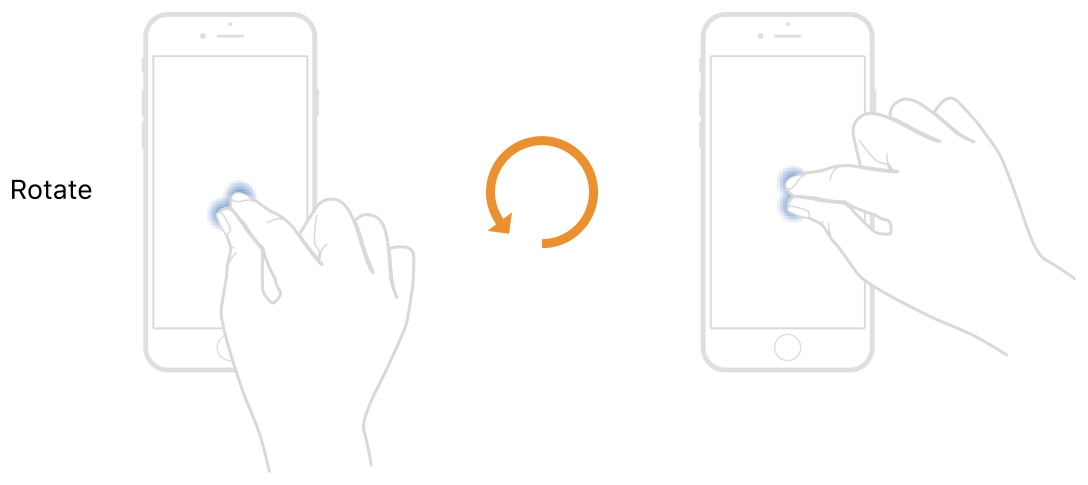
\includegraphics[width=0.7\textwidth]{Research-Latex/images/touchscreenGestures.png}
     \caption{iPhone Touch Screen Gesture Recognition }
\end{figure}
  
  \item \textbf{Camera Gestures:}Camera gestures refer to the use of users interacting with their device by the device's camera implementing methods for accessing functionality via mathematical algorithms. Use cases range from pause,  start and sleep functions, etc instead of using traditional hardware. Hand detection plays a huge road in recognizing gestures inside of the camera sensors. The automobile giant BMW has included a gesture recognition system for the dashboard by using a 3D Camera and deep learning algorithms to model the user's movement into gestures. Sample gestures included are as follows:
  
 \begin{flushright}
  \begin{itemize}
	\item Accepting a Call  / Confirming pop-up: Point one finger towards the iDrive screen and pull it back
	\item Rejecting a Call / Closing pop-up: Swipe your hand to the right 
Turning up the volume: Circle your finger clockwise
\end{itemize}
   \end{flushright}

  
  
  \begin{figure}[h!]
  \centering
    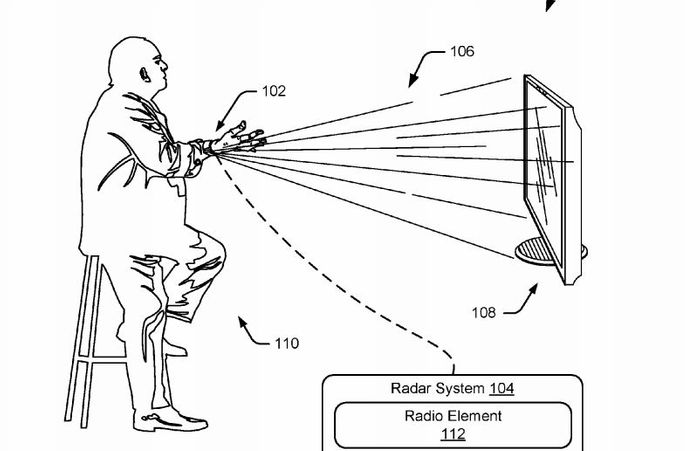
\includegraphics[width=0.5\textwidth]{Research-Latex/images/googleCameraRecognition.jpeg}
     \caption{Camera Gesture Recognition }
\end{figure}




  \item \textbf{Voice Gestures:} Voice gestures refer to the use of users interacting with their device by the device's microphone implementing methods for accessing functionality as pause,  start and sleep functions, etc. Prime examples of devices that implement voice recognition are Microsoft's ' Cortana ' assistant and Apple's voice assistant 'Siri' released in October 2011 now turns a decade old but still offers a near-identical interface.
  
\textbf{Interacting with voice Assistants  Siri and Cortana}


  \begin{itemize}
  	\item \textbf{Example Siri Commands }
  		\item Siri is exclusive to the Apple ecosystem 

	\item "Hey Siri" - Activates voice assistant 
	\item "What's the weather today? - Reads weather forecast based on location
	\item 	"How many cups are in a quart?" -  mathematical question

	

\end{itemize}

\begin{itemize}
  	\item \textbf{Cortana Commands }
  	  		\item Cortana is exclusive to the Microsoft  ecosystem 

	\item click the Cortana button to the right - Activates voice assistant 
	
\end{itemize}
  \begin{figure}[h!]
  \centering
    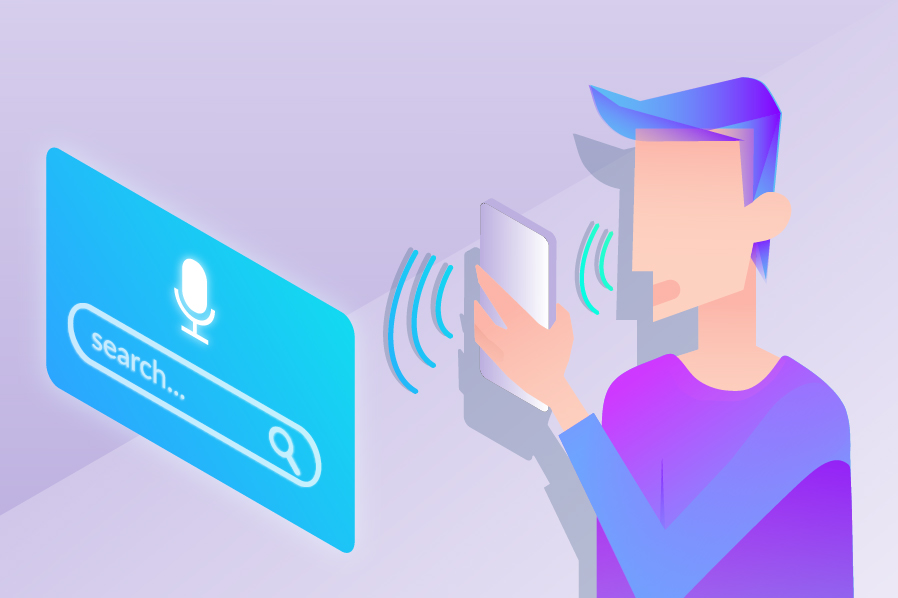
\includegraphics[width=0.5\textwidth]{Research-Latex/images/voiceRec.jpg}
     \caption{Voice Gesture Recognition between user and smart device }
\end{figure}



\end{itemize}



  
  
  
\subsection{Gesture Systems}
Gesture recognition is made possible through the use of artificial intelligence. Wikipedia defines AI as' Artificial intelligence (AI) is intelligence demonstrated by machines'.




\subsection{Gesture  Suitability }

A large issue is how companies can overcome incorporating their gestures into current systems. Users are used to interacting with their devices in a hardware orientated manner such as turning the volume up with a volume controller. The motor industry is a prime example of a sector that is highly monitored and companies must meet standard regulations on e.g side mirrors, windscreens, etc. One area companies fell in implementation is the suitability of the gestures. Consumers want a simple user and will only use gestures if it is easier or faster. I too have felt defeated to use a new gesture on console or tablet due to simply the hardware is easier to use and have already know the Ins and Outs of the device. 


\subsection{Current market }
As discussed in section 2.0.4 ' the video game Industry ' The Xbox Kinect at launch in 2010 was a wide success but was short-lived by the current market. The device was great for activity-orientated games such as boxing, bowling, etc but it failed in the juggernaut areas such as First Person shooters like Call of Duty and Medal of Honour. Currently an expanding market. The vast amount of funding needed to create gesture systems is not worth time and finance if the market share is not big enough. The current generation of consoles (PlayStation 5, Xbox One) all provide gesture-based equipment such as via camera and handheld equipment with unique software. There has been an absence of gestures in multimedia players and e-reader devices due to its poor market share. Over the last decade, there has been a leap in gesture technology in medicine, University ' Ben Gurion has developed  a ' hand-gesture recognition system that enables doctors to manipulate digital images during medical procedures using hand gestures instead of touch screens or computer keyboards.' This is a massive achievement and due to the Covid-19 pandemic, this could become a new way to interact with reports in offices and the workplace.

